%%%%%%%%%%%%%%%%%
% Configuration %
%%%%%%%%%%%%%%%%%


\documentclass[twocolumn]{article}
\usepackage{geometry}
\geometry{twoside=true, head=13pt,
     columnsep=2pc,
     top=57pt, bottom=73pt, inner=54pt, outer=54pt,
     marginparwidth=2pc
 }
\usepackage{libertine}
\usepackage{newtxmath}
\usepackage{inconsolata}

\usepackage{adjustbox}
\usepackage{enumitem} \setlist{leftmargin=*}
\usepackage[english]{babel}
\usepackage{array}
\usepackage{xurl}
\usepackage[super,comma,sort&compress]{natbib}
\usepackage{enumerate}
\usepackage{hyperref}
\usepackage{amsmath}
\usepackage{booktabs}
\usepackage{multirow}
\usepackage{csquotes}
\usepackage{hhline}
\usepackage{caption} \captionsetup{justification=centering}
\usepackage{float}
\usepackage[multiple]{footmisc}
\usepackage[LGR,T1]{fontenc}
\usepackage[utf8]{inputenc}
\usepackage{dblfloatfix}
\usepackage{threeparttable}

\newcommand{\textgreek}[1]{\begingroup\fontencoding{LGR}\selectfont#1\endgroup}

\newcommand{\nullhypothesis}[1]{
\vspace{-0.5em}
\begin{itemize}[label=$H_0$:]
\item #1
\end{itemize}
}

\usepackage[backend=biber,style=numeric,sorting=nty]{biblatex}
\bibliography{references.bib}

\usepackage{graphicx}
\graphicspath{ {images/} }

\def\code#1{\texttt{#1}}
% \def\shortcite#1{\citetitle{#1} (\citeauthor{#1}, \citeyear{#1})}
\def\shortcite#1{\citetitle{#1}. \citeauthor{#1}, \citeyear{#1} \cite{#1}}

\def\bolditem#1{\item\textbf{#1:}}

% Load required packages
\usepackage{titlesec} % For customizing section titles

% Define a new counter for the special subsubsections
\newcounter{methodcounter}[section] % Reset counter at each new section

% Set the representation of the methodcounter to uppercase letters
\renewcommand{\themethodcounter}{\Alph{methodcounter}}

% Define the \method command
\newcommand{\method}[1]{
  \refstepcounter{methodcounter}
  \subsubsection*{\normalsize \themethodcounter. #1 \vspace{-0.5em}}
}

\newcommand{\centerimg}[1]{
  \begin{adjustbox}{center} #1 \end{adjustbox}
}

\newcounter{rqcounter}\setcounter{rqcounter}{-1}
\newcommand{\researchquestion}[1]{
  \refstepcounter{rqcounter}
  \begin{itemize}[label=\textbf{RQ\therqcounter}:]
  \item #1
  \end{itemize}

}

\newcommand{\sig}{$\ast\!\ast\!\ast$}
\newcommand{\nonumitem}{\item[]\hspace{-\leftmargin}}


% Make float placement less strict
\renewcommand{\textfraction}{0.05}
\renewcommand{\topfraction}{0.9}
\renewcommand{\bottomfraction}{0.9}
\renewcommand{\floatpagefraction}{0.85}


%%%%%%%%%%%%
% Document %
%%%%%%%%%%%%
\title{Topic Analysis of Textbooks Using AI}
\author{
    Coby B. Simmons \\
    \small{\href{mailto:cobysimmons01@gmail.com}{cobysimmons01@gmail.com}}
}
\date{
    Utrecht University\\%
    The University of Sydney\\[2ex]%
    February 2024
}

\begin{document}

\maketitle

\section*{Abstract}
Advances in the field of artificial intelligence (AI) and natural language processing (NLP) have opened new horizons for personalised learning.
It has been shown that online learning platforms are tremendously beneficial in promoting student engagement. Given the widespread use of textbooks in the learning process and the limited technological advancements that have been made with regard to their use, it is worth exploring how textbooks can be leveraged to enhance the learner's experience in the growing trend towards online learning.
This research focuses on the applications, of AI in identifying and categorising topics within educational content. 
Specifically, we aim to construct comprehensive models that accurately reflect the depth and breadth of a particular domain using the knowledge embedded in textbooks. These domain-specific and fine-grained topic models will be used to generate a dataset for the training of state-of-the-art deep learning models to identify the topics present in new pieces of text.
Our motivation is that a dense and comprehensive domain model based on textbooks can serve as a sophisticated framework for educational applications, enabling them to provide enhanced learning experiences via downstream tasks such as learning object classification, automatic index creation, and content personalisation.
Thus, we propose an architecture that moves away from classic, unsupervised topic modelling techniques and attempts to implement a fine-grained, semi-supervised approach.


\textbf{Keywords:} \quad textbooks, semantic linking, natural language processing, deep learning, semi-supervised learning, topic classification

\section{Introduction}

The advent of online learning has brought about a ground-breaking transformation in education, offering unparalleled opportunities to learners worldwide. It has been shown that online learning platforms are tremendously beneficial in promoting student engagement \cite{benta2014}. Given the widespread use of textbooks in the learning process \cite{kumar1986}, it is worth exploring how they can be leveraged to enhance the learner's experience in the growing trend towards online learning.

Work to bring textbooks into the digital age has already been undertaken. Specifically, there exists online learning platforms that incorporate improved search and navigation functionalities \cites{dichev2006,sosnovsky2014,brusilovsky1998,brusilovsky2007} and interactive content \cite{ericson2019}. However, in practice, these methods are typically heuristic and do not necessarily take advantage of AI. Additionally, for most textbooks, the digital and printed versions are identical. This may be because the AI models underlying these e-learning approaches do not exhibit the high level of performance required for acceptance in the rigorous domain of education.

For AI to perform effectively on education-related tasks, it is necessary to construct a domain-specific, fine-grained topic model. ``Domain-specific'', in this context, emphasises that concepts or knowledge are unique in their definition for a particular domain \cite{sekine1997}. Consider the concept of ``mean'' as an example. In the statistics domain, the mean is typically related to probability distributions, statistical inference, the Central Limit Theorem, and so on. In finance, however, the concept is more closely associated with the notions of risk or time value of money. Given that textbooks (and other learning objects) are generally limited to their respective domains, this research investigates whether domain-specificity can help improve the accuracy and efficiency of AI models by imparting a better understanding of relevance.

Working in conjunction with domain-specificity is the notion of fine granularity. In the context of topic models, fine granularity refers to the detailed and specific division of topics, where the model identifies and differentiates between closely related subtopics rather than grouping them under broad, general categories. This approach allows for a more precise and nuanced understanding of the content, enabling the identification of subtle distinctions and variations within the data. 

A domain-specific, fine-grained topic model may not be essential for broader applications of classification. For example, when classifying topics in news articles, the topics tend to be broader and less nuanced (e.g. politics, sports, business), allowing for easy classification without the need for deep, specialised analysis \cite{lee2011}.

Conversely, academic texts often delve into complex and highly specialised topics, where differences are subtler and lexical overlap is significant \cites{alpizarchacon2022,yang2018}. This level of detail requires a fine-grained approach to accurately classify and organise content according to its precise academic domain, facilitating better inference outcomes. Thus, our research is based on the premise that domain-specific, fine-grained topic models are essential in capturing the depth and breadth of subjects in textbooks.


Our motivation is that a dense and comprehensive domain model based on textbooks can serve as a sophisticated framework for educational applications, enabling them to provide enhanced learning experiences via downstream tasks such as learning object classification, automatic index creation, and content personalisation. This application of AI in education has the potential to revolutionise the way we teach and learn, making education more efficient, effective, and accessible for all.

Given this, our overarching research question is 
\researchquestion{
What is the efficacy of training fine-grained, domain-specific topic models from textbooks using machine learning methods?
}

We explore the optimal configuration for such an approach with three sub-research questions, the first of which is
\researchquestion{
Which topic modelling techniques perform best in linking content to construct a topic hierarchy?
}

This content linkage process leads to the creation of a fully integrated textbook that covers the breadth and depth of a particular domain. This ``joint hyperspace of cross-linked textbooks'' is introduced to address issues such as subjectivity, limited scope and inadequate detail that may arise in individual textbooks, thus resulting in ``a more complete and objective model'' \cite{alpizarchacon2020}.

This comprehensive and unified data collection can be normalised and then used to train deep learning models to classify topics within the domain of choice. We consider the conditions that lead to optimal performance in this stage of the process with two more sub-research questions:
\researchquestion{
How does the performance of deep learning models vary when additional semantic information (i.e. concept annotations) is included in the data?
}
\researchquestion{
How does the performance of deep learning models vary across datasets with different levels of quality?
}

This research shows that topic models extracted from the hierarchy of textbooks perform better than the baseline at classifying new textbook sections into topics, particularly when additional semantic information is included in the data. Our proposed method for automatic content linkage demonstrated promising results, achieving a performance level that, while not yet matching the precision of experts' manual efforts, shows significant potential. It's important to note that there was a decrease in topic classification accuracy when utilising the automatically generated topic model, suggesting areas for further refinement.

The rest of this paper is organised as follows: Section~\ref{sec:background} provides an overview of the existing research in this space, with a particular focus on the methods that we will apply. In Section~\ref{sec:methodology}, our methodology is further discussed with a detailed proposal for an architecture that can be used to answer our research questions. Our results are explored and evaluated in Section~\ref{sec:results} and they are discussed in Section~\ref{sec:discussion}. Finally, Section~\ref{sec:conclusion} summarises the paper and indicates some areas for future research.

\section{Background} \label{sec:background}

\subsection{Modelling of Textbooks} \label{sec:modelling-of-textbooks}

Previous works have explored the transformation of PDF textbooks into interactive and intelligent online learning materials \cites{alpizarchacon2019,alpizarchacon2021,alpizarchacon2020, alpizarchacon2022}. Figure~\ref{fig:alpizar-chacon-workflow} broadly summarises these works as a single automatic workflow that has been developed to extract knowledge models for PDF textbooks.

\begin{figure*}[h!]
\caption{Textbook knowledge model construction workflow from \textcite{alpizarchacon2020}}
\centerimg{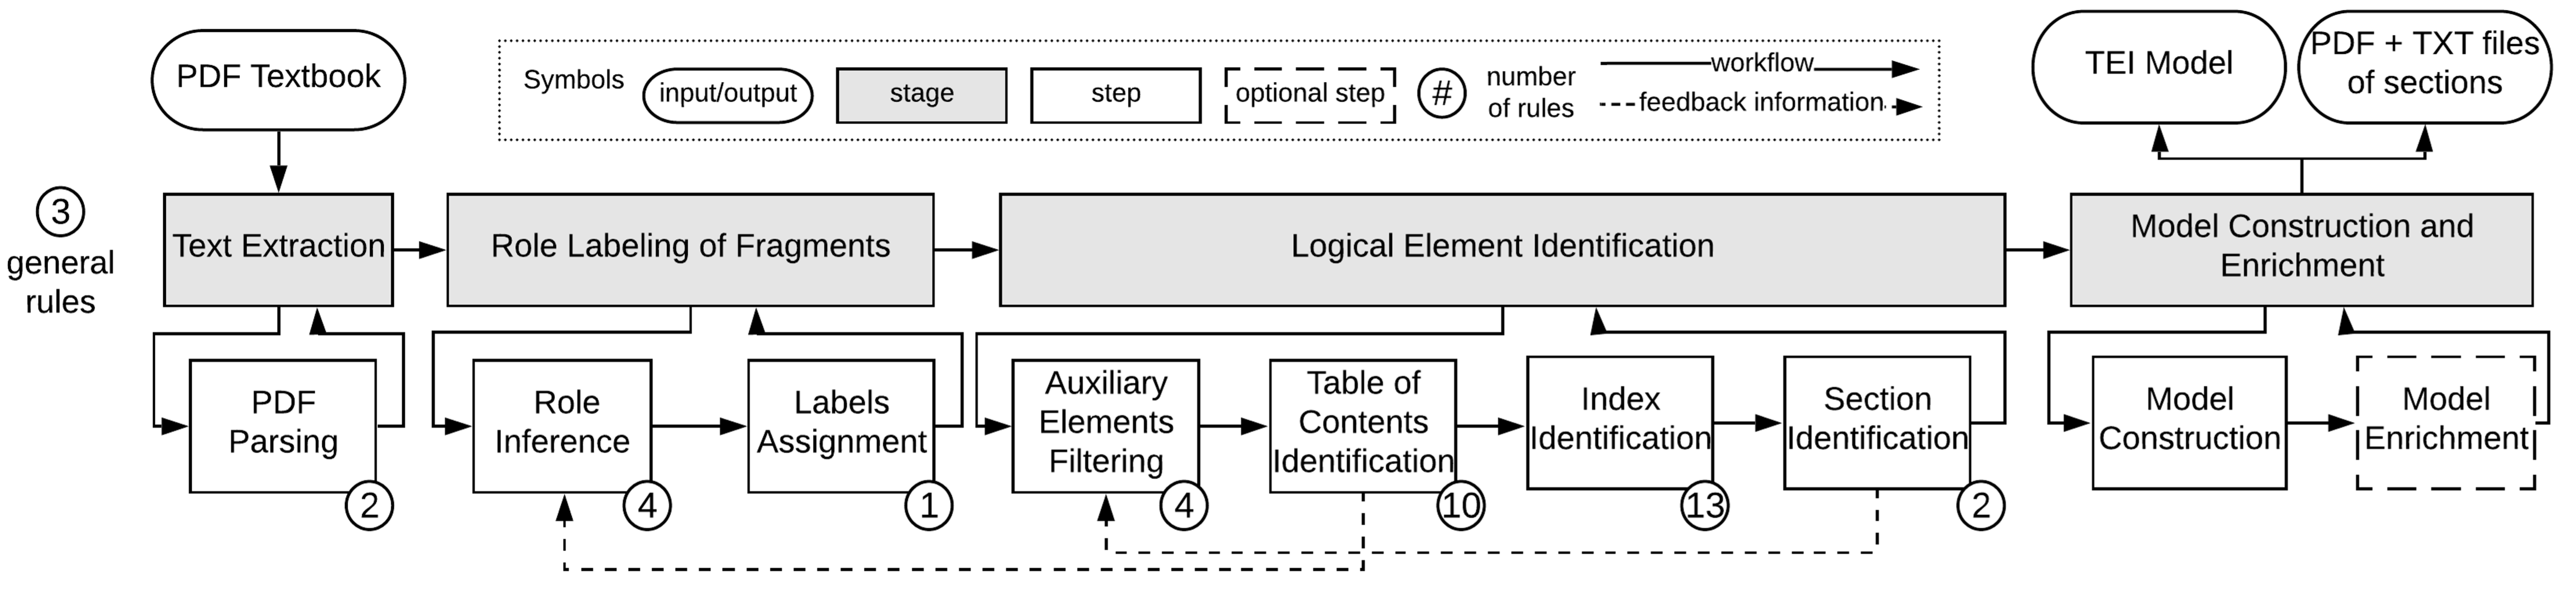
\includegraphics[width=\textwidth]{alpizar-chacon-workflow.png}}
\label{fig:alpizar-chacon-workflow}
\end{figure*}


First, a comprehensive set of rules is defined to capture the typical conventions in the formatting, structure, and organisation of textbooks. Key elements such as the structure of the textbook (including chapters and subchapters), content (consisting of words, lines, text fragments, pages and sections) and domain-specific terms are extracted.

The workflow then uses the domain terms to connect to DBpedia, a large-scale knowledge base extracted from Wikipedia \cite{lehmann2015}. The linkage of glossary terms to DBpedia facilitates the enrichment of these terms with semantic information such as concept definitions and categories (see Section~\ref{sec:methodology} for more detail), thus improving the quality of the domain terms, broadening their contextual understanding, and connecting the textbooks to the Linked Open Data Cloud.

Finally, the extracted knowledge is serialised according to the Text Encoding Initiative (TEI) Guidelines\footnote{\url{https://www.tei-c.org/release/doc/tei-p5-doc/en/html/index.html}} and the resulting files are used as the input for this research (see Section~\ref{sec:data}).

The TEI Guidelines establish a unique XML-based format that predominantly focuses on the semantic aspects of the textbook, unlike other open file formats that focus more on presentation (e.g. HTML, PDF, etc.). The framework encompasses around 500 distinct textual elements (e.g. words or glyphs) and concepts (e.g. names or definitions).

Furthermore, ``back-of-the-book indices'' are explored for the benefits that they provide in information retrieval and knowledge organisation since they provide a collection of important domain terms curated by experts. The research presents a method for enriching the knowledge model of textbooks, by classifying each index term according to their relevance to a particular domain. Each term can be classified as
\vspace{-0.6em}\begin{itemize}\itemsep-0.3em
    \item \textbf{core-domain:} index terms representing the most important and frequent concepts in the domain;
    \item \textbf{in-domain:} additional index terms in the domain;
    \item \textbf{related-domain:} index terms tangential to the domain;
    \item \textbf{out-of-domain:} index terms not related to the domain (e.g. from examples).
\end{itemize}\vspace{-0.6em}

This annotation of concepts found in the index can be exploited to aid in the modelling of textbook topics. By incorporating these concepts, which succinctly capture the essence of each section, the model gains access to a concise summary that highlights the main ideas. This additional layer of information is anticipated to improve the model's ability to accurately identify and weigh the significance of crucial terms within the text \cite{alpizarchacon2023a,alpizarchacon2023}.

While the above workflow describes the construction of a textbook knowledge model, it does not specify how learners might be able to access this knowledge effectively and engagingly. Thus, a proposal is made for `Intextbooks', an intelligent and personalised online learning experience \cite{alpizarchacon2020intextbooks}. In this proposal, `semantic markup' is closely integrated with a presentational representation of the PDF textbook to provide a platform where a learner can not only view a given textbook, but can also jump to different sections, search for occurrences of a word, and access enriched semantic information that is external to the textbook itself. Aside from providing a user interface for the domain and content model, a user might be able to have conversations with other users or annotate the textbook's content with highlights, bookmarks, and notes. Thus, Intextbooks results in an e-learning platform that enriches the simple and somewhat featureless PDF textbook. 

\subsection{Topic Modelling \& Semantic Similarity}

In his foundational treatise on logic and argumentation, \textit{Topics}, Aristotle develops a system of `places' – mental locations or categories – where different types of arguments could be found and utilised. Thus, the term `topic' comes from the Greek \textit{tópos} (\textgreek{τόπος}), meaning `place' or `locus' \cite{oed:topic}.

Topics can be formed and detected through a variety of processes, but perhaps the most significant source is through inquiry and discourse. They are often shaped by the way we describe and talk about phenomena. Textbooks are the ultimate resource for these processes \cite{ramnarayan2003}. Thus, they can serve as an effective input into the modelling of topics \cite{alpizarchacon2020}.

Mathematical concepts like vectors and probability can be used to model the abstract structure of topics, just as they can be used to model other spaces (both physical or abstract) \cite{churchill2022}. These ``vector space or semantic space models of meaning'' underlie nearly all modern methods in semantics that involve corpus analysis \cite{bruni2014}. Thus, a word's meaning is represented by a vector that records frequency and co-occurrence patterns within text corpora.

Semantic similarity refers to the degree to which two pieces of text are alike in meaning \cite{mohammad2012}. Within the aforementioned frameworks, the similarity between two or more words can be accurately measured by a geometric comparison of the vectors that represent them. The cosine similarity metric is used in this research since it has been shown previously to be a very effective measure of semantic similarity \cite{bullinaria2007}.

Given two $n$-dimensional semantic vectors, $\textbf{a}$ and $\textbf{b}$, the cosine similarity $S_C$ is the dot product of the vectors, divided by the product of their lengths. Additionally, cosine similarity can also be thought of as the angle $\theta$ between the two vectors. Both interpretations are shown in Equation~\ref{eq:cos-sim}.

\begin{equation}\label{eq:cos-sim}    
S_C(\textbf{a}, \textbf{b}) := \cos(\theta) = \frac{\textbf{a} \cdot \textbf{b}}{\|\textbf{a}\| \|\textbf{b}\|}
\end{equation}

Thus, the directions of the two vectors serve as a proxy for their semantic content. A cosine similarity of $0$ indicates orthogonal vectors, representing no semantic similarity. A cosine similarity of $1$ or $-1$ indicates parallel vectors, representing semantic content is perfectly similar or perfectly opposite, respectively.

Cosine similarity is unaffected by the magnitude of vectors, a particularly useful property in text analysis where the length of documents can vary greatly.

In recent years, various techniques for unsupervised topic discovery have been introduced. The most relevant of these techniques are outlined in the remainder of this section.

\subsubsection{Term Frequency-Inverse Document Frequency (TF-IDF)}

TF-IDF is a statistical measure used to evaluate the importance of a word in a document, in relation to the document’s corpus.
The Term Frequency (TF) component measures the frequency of a word in a specific document, essentially representing the importance of the word in understanding the document's content.
The Inverse Document Frequency (IDF) component is the logarithmically-scaled, inverse of the frequency of documents in the corpus that contain a particular term, penalising terms that appear in many documents, as they are less valuable in distinguishing between documents \cite{sparckjones1972}. Thus, for a term $t$ in a document $d$ in a corpus of size $N$, the TF-IDF is
\begin{equation}
    {t\!f}_{t,d} \times \log\frac{N}{{df}_t}
\end{equation}
where ${t\!f}_{t,d}$ is the frequency of $t$ in $d$ and ${df}_t$ is the number of documents containing $t$.

\subsubsection{Latent Semantic Indexing}

Latent Semantic Indexing (LSI) is another foundational technique in the development of topic models \cite{deerwester1990}. At its core, LSI aims to identify patterns in the relationship between terms, documents, and concepts that simple term matching cannot pick up. For example, TF-IDF often fails to account for nuances like synonyms or context.

These latent semantic structures are uncovered by applying Singular Value Decomposition (SVD) to the original term-document matrix. SVD decomposes this matrix into three smaller matrices, representing the relationships between documents, terms, and the concepts they imply. These matrices are then recombined in a way that retains most of the significant information while discarding noise and less important details. The essential patterns captured in this reduced matrix reveal how terms and documents are related in terms of underlying topics or concepts. By focusing on these patterns rather than just exact term matches, LSI more effectively aligns queries with relevant documents, improving the accuracy of information retrieval.

\subsubsection{Latent Dirichlet Allocation} \label{sec:lda}

Latent Dirichlet Allocation (LDA), an extension of LSI, was introduced by \textcite{blei2003} as a generative probabilistic model for topic modelling. In LDA, each topic is defined by the likelihood of each word appearing in that topic (e.g. the topic `physics' might assign higher probabilities to words like `quantum', `energy', or `particle'). In turn, documents are modelled as as mixture of topics (e.g. a document in a collection of academic texts might be 30\% about physics, 50\% about mathematics, and 20\% about computer science).

In \textcite{guerra2013}, LDA was used to link documents from different textbooks. It was found to be more effective than a baseline method that uses Apache Lucene based on the TF-IDF model.

However, a significant issue with LDA is the need to predefine the number of topics. This parameter can vary greatly for different types of datasets and can also significantly influence the model's performance and the coherence of the topics generated. Furthermore, LDA may produce poor-quality topics when documents have overlapping or tangential topics \cite{ajinaja2023}.

\subsubsection{Embedding Models}

In recent years, embedding models have revolutionised the field of topic modelling, moving beyond traditional methods that treat words and topics as discrete, atomic units. These models create dense vector representations of words and documents, capturing semantic relationships in a continuous vector space, and thus providing a more sophisticated and contextually aware approach to understanding language and text data.

Word2Vec is a pivotal example of this approach \cite{mikolov2013}. It generates vector representations for words in such a way that the spatial relationships between vectors capture semantic relationships between words. For instance, in this vector space, words with similar meanings, like `apple' and `banana,' are positioned closer together than unrelated words like `elephant.' Word2Vec also excels at capturing analogies; for example, the relationship between `king' and `queen' is analogous to that between `man' and `woman' in its vector space.

Extending this concept to documents, Doc2Vec allows entire documents to be represented as vectors \cite{le2014}. This method enables the comparison of documents in a multi-dimensional vector space that considers the overall context and semantic content of the documents, not just isolated word usage. Doc2Vec outperforms LDA in textbook content linkage tasks \cite{thaker2018}.

Another significant advancement in this field is Top2Vec \cite{angelov2020}. Top2Vec builds upon the principles of Word2Vec and Doc2Vec by creating joint embeddings of words and documents. It automatically detects topic vectors in the joint word and document embedding space. Each detected topic is represented as a dense vector in this space, and documents and words closest to this vector are most relevant to the topic. This approach allows for a more intuitive and semantically rich way of understanding and categorising documents and topics. It effectively captures the nuances of language and thematic structures within large text corpora.


\subsection{Advanced Language Models}
In recent years, more powerful and advanced language models have become available.

\subsubsection{Bidirectional Encoder Representations from Transformers}

\begin{figure*}[h!]
\caption{Diagram of the BERT pre-training and fine-tuning stages}
\centerimg{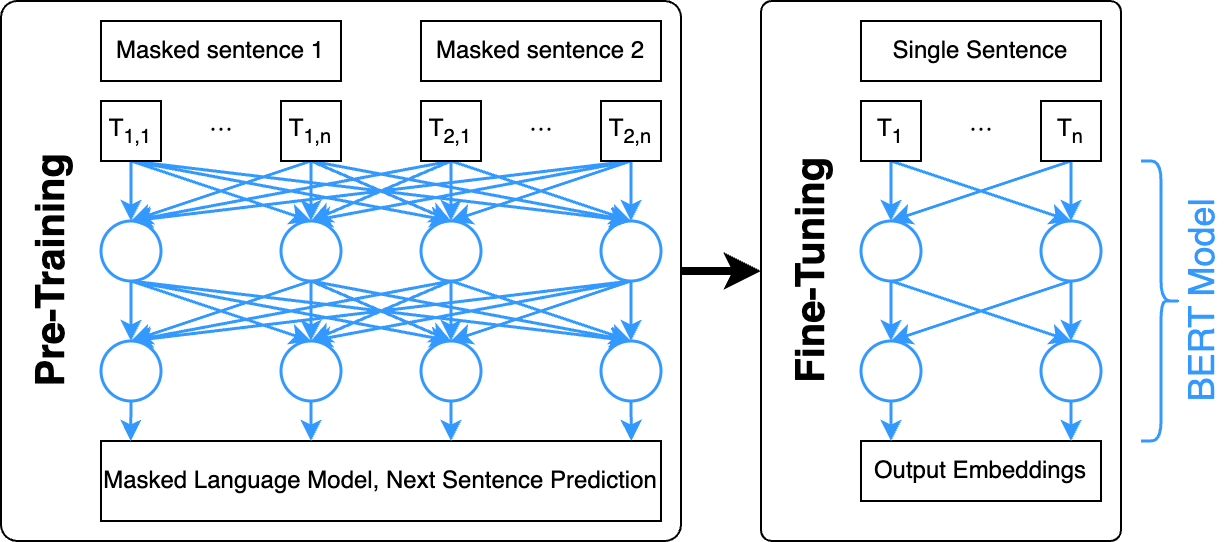
\includegraphics[width=0.8\textwidth]{bert.png}}
\label{fig:bert}
\end{figure*}

In \textcite{devlin2019}, Bidirectional Encoder Representations from Transformers (BERT) are introduced as a ``language representation model'' that operates bidirectionally, i.e. it can understand the context of words in a sentence from both the left and right directions. This represents a significant leap forward from previous models that perceive text unidirectionally.

The lifecycle of preparing a BERT model for an NLP task is divided into the pre-training and fine-tuning stages. These processes are displayed graphically in Figure~\ref{fig:bert}.

BERT is unique in its approach to pre-training, which involves two unsupervised tasks. It uses masked language modelling, where some percentage (usually 15\%) of input tokens are replaced by random masking and the model is trained to predict these masked tokens. Additionally, BERT utilises a next-sentence prediction (NSP) task to determine if a sentence follows the previous one in the original document. This method enables the model to understand sentence relationships and context, which is crucial for many downstream tasks. Pre-training typically uses a large corpus of texts (e.g. Wikipedia). It can take hours to days and requires significant computing power. Thus, various open-source pre-trained models are available for download \cite{huggingface}.

In the fine-tuning phase, the pre-trained BERT model is adjusted to a more specific NLP task (e.g. sentiment analysis, question answering, or document classification).
This involves adjusting the model's weights slightly to tailor it to the nuances of the task at hand, leveraging the general understanding of language that the model gained during pre-training. Fine-tuning is typically performed on a smaller, narrower, labelled dataset.

BERT has been shown to achieve state-of-the-art performance when the language embeddings that it generates are used as input features for downstream NLP tasks.

In the education domain, the rich data potential of textbooks has been harnessed by using BERT to develop a tool for automatic keyword extraction, thus providing a cost-effective and efficient alternative to traditional manual data annotation methods \cite{alpizarchacon2023a}. Given the existing workflow for textbook knowledge model extraction described in Section~\ref{sec:modelling-of-textbooks}, this approach leverages textbook indexes to extract domain-specific knowledge that can be used to label datasets, which in turn can be used for downstream supervised learning tasks.

It is important to note that BERT is extremely computationally intensive. To mitigate this, research was undertaken to develop a method to pre-train a distilled version of BERT (DistilBERT) \cite{sanh2020}. It was shown that DistilBERT can result in a BERT model that is 40\% smaller and 60\% faster while retaining 97\% of the language understanding capabilities of the original model.

\subsubsection{Recurrent Neural Networks}

Recurrent Neural Networks (RNNs) are a type of deep neural network that functions as a dynamic system, possessing a distinct internal state at every stage of the classification process \cite{staudemeyer2019}. This unique characteristic stems from self-feedback loops within the network, which facilitate the transfer of information from previous occurrences to the current processing stages. Consequently, RNNs develop a capacity to remember sequences in the data.

However, RNNs can face the ``vanishing gradient problem'', whereby the gradient of the loss function becomes too small for effective learning, making it difficult for the network to learn long-range dependencies \cite{bengio1994}.

Additionally, the sequential nature of RNNs means they cannot be easily parallelised, leading to longer training times compared to other architectures. While RNNs can theoretically remember long sequences, in practice, they often struggle with dependencies that are separated by long intervals in the data.

Long Short-Term Memory (LSTM) networks were introduced to overcome the limitations of traditional RNNs, particularly the vanishing gradient problem \cite{hochreiter1997}. This is achieved through the introduction of a structure called a memory cell, capable of maintaining information in memory for long periods. The key to this capability is the use of gates that regulate the flow of information into and out of the cell, thereby addressing the vanishing gradient problem and preserving long-term dependencies in sequential data more effectively than traditional RNNs. 

\subsection{Linking Multiple Textbooks}

\textcite{guerra2013} describes two methods for handling the hierarchical structure of the textbook, which can be applied to our vector representations of documents:
\begin{enumerate}[a)]
    \item \textbf{Topic Aggregation:} Only compute the topic vectors for the sections at the lowest level in the hierarchy, and for higher levels, aggregate topic vectors by taking a weighted average of sub-topic vectors.
    \item \textbf{Re-Indexing:} Compute the topic vector for every section by considering a section's `document' to be the content of the section and all its sub-sections.
\end{enumerate}

The Topic Aggregation method is much more computationally efficient since vectors do not need to be recomputed regularly. Thus, it is the approach taken for this research.

\subsection{Topic Classification}


Topic classification involves categorising texts or documents into predefined topics or classes. Typically, this classification has been performed across broad and distinctly separate areas (e.g. such as technology, sports, and science) with considerable success \cite{lee2011}. Such categorisation leverages the clear conceptual and lexical differences between categories, facilitating the development of models that can accurately differentiate based on distinct features and terminologies inherent to each domain. As described in Section~\ref{sec:lda}, LDA is primed to perform well under these conditions and there is evidence of this \cites{lancichinetti2014, li2016}.

However, challenges emerge when topic classification is applied within a single, homogeneous domain, where the distinctions between subtopics are subtler and the lexical overlap is significant. Fine-grained classification seeks to distinguish between smaller, more specific categories that fall under a broader parent domain \cite{yang2018}. These specific categories are generally defined by domain experts using intricate criteria, which generally focus on subtle differences. Synthesising these definitions is a time-consuming task. However, we propose that the hierarchy of textbooks can effectively be translated into a model of the topics in a domain. Through the content linkage process defined in Section~\ref{sec:content-linkage}, a comprehensive and unified data collection for a particular domain is generated, thus removing the need for resource-intensive, fine-grained human annotations.

\subsection{Summary}

Inspired and informed by the related works summarised in Table~\ref{table:related-works}, we aim to contribute to the field of AI in education through our proposal of a new architecture. This architecture builds upon principles used in fine-grained image classification to generate a labelled dataset with minimal human intervention that is then used as the input for a domain-specific topic classification model.

\begin{table*}[h!]
\centering
\caption{Summary of related works}
\label{table:related-works}
\small
\begin{tabular}{ll}
\toprule
reference & contribution \\
\midrule
\textcites{alpizarchacon2019,alpizarchacon2020, alpizarchacon2021,alpizarchacon2022} 
    & extracting knowledge models from textbooks \\
\textcite{alpizarchacon2020intextbooks} 
    & intelligent online learning experience \\
\textcite{ramnarayan2003} 
    & textbooks as an effective source for topic modelling \\
\textcite{bullinaria2007} 
    & effectiveness of cosine similarity in measuring semantic similarity \\
\textcite{guerra2013} 
    & effectiveness of LDA in linking topics from textbooks \\
\textcite{thaker2018} 
    & improved performance of Doc2Vec over LDA in textbook content linkage tasks \\
\textcite{alpizarchacon2023a} 
    & use of BERT for automatic keyword extraction from textbooks \\
\textcites{lancichinetti2014, li2016} 
    & effectiveness of LDA in classifying content into broad topic areas \\
\textcite{yang2018} 
    & fine-grained image classification \\
\bottomrule
\end{tabular}
\end{table*}


\section{Methodology} \label{sec:methodology}

This section proposes our methodology for the extraction of fine-grained, domain-specific topic models from textbooks to answer \textbf{RQ0}. Our motivation for this method is that it is a quick and inexpensive way to develop a dataset that provides a rich and fine-grained representation of a particular subject area. We propose a pipeline that fits broadly into two phases.

In Phase 1, we aim to construct a hierarchy of topics within a domain using various topic modelling techniques. To achieve this, we first parse the textbook knowledge models obtained using the processes described in previous research (see Section~\ref{sec:modelling-of-textbooks}). This parsing process involves extracting the position of each section in the textbook hierarchy. Additionally, the following five key attributes are extracted for each section:
\begin{itemize}\itemsep-0.2em
    \item \textbf{header}: the title of the textbook section (e.g. ``Measures of Location'')
    \item \textbf{content}: the textual content associated with each section (e.g. ``Visual summaries of data are excellent tools for obtaining preliminary impressions and insights...'') 
    \item \textbf{concept names}: the DBpedia resources referenced in the textbook section (e.g. ``Coefficient of variation'')
    \item \textbf{concept definitions}: the definitions associated with DBpedia resources referenced in the textbook section (e.g. ``In probability theory and statistics, the coefficient of variation is a ...'')
    \item \textbf{concept subjects}: the category of DBpedia resources referenced in the textbook section (e.g. ``Statistical deviation and dispersion'' for concept ``Coefficient of variation'').
\end{itemize}
Only concepts marked ``core-domain'' and ``in-domain'' are included. This is to avoid confusing the models with extraneous data. The definitions for domain specificity are provided in Section~\ref{sec:modelling-of-textbooks}.

After parsing, the topic modelling methods are applied to the parsed textbook data and the performance of each technique is evaluated to address \textbf{RQ1} and choose an optimal technique. Using the best method, a comprehensive and unified data collection is generated from the textbook knowledge models and then converted into a normalised, labelled dataset.

Phase 2 involves the conversion of the labelled dataset into vector embeddings, and then the use of these vectors to train supervised deep learning models. \textbf{RQ2} explores the differences in performance seen in this phase when concept annotations are included in the input, while \textbf{RQ3} explores the differences in performance due to different dataset generation methods tested in Phase 1.

Figure~\ref{fig:architecture} presents this methodology graphically, showing the various sub-parts of each phase and the prerequisite data for the pipeline.

\begin{figure*}[h!]
\caption{Architecture for topic representation and classification}
\centerimg{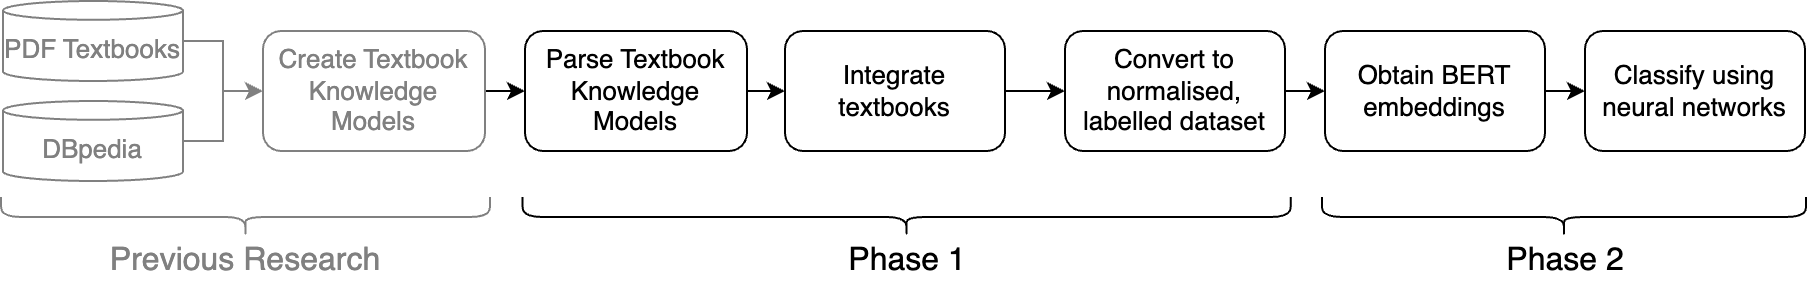
\includegraphics[width=1.05\textwidth]{simple-architecture-new.png}}
\label{fig:architecture}
\end{figure*}

\subsection{Phase 1: Dataset Generation} \label{sec:dataset-generation}

\subsubsection{Data} \label{sec:data}

In this research, twelve textbooks from the statistics domain were used to develop our method:
\begin{itemize}\itemsep-0.2em
    \item \code{BookA}: \shortcite{devore2011}
    \item \code{BookB}: \shortcite{walpole2010}
    \item \code{BookC}: \shortcite{dekking2005}
    \item \code{BookD}: \shortcite{madsen2011}
    \item \code{BookE}: \shortcite{kaltenbach2011}
    \item \code{BookF}: \shortcite{finkelstein2009}
    \item \code{BookG}: \shortcite{faber2012}
    \item \code{BookH}: \shortcite{shanmugam2015}
    \item \code{BookI}: \shortcite{uboe2017}
    \item \code{BookJ}: \shortcite{wolfe2017}
    \item \code{BookK}: \shortcite{diez2019}
    \item \code{BookL}: \shortcite{dalgaard2008}
\end{itemize}

From this set, a base textbook is chosen and used as a foundation to hierarchically integrate the sections from other textbooks, such that the result is a table of contents where each entry points to groups of sections rather than a single section.

We chose \code{BookA} as the base textbook for two key reasons. Firstly, there exists an expert-generated mapping between the sections of \code{BookA} and \code{BookB} that can be used to evaluate the textbook integration methods (see Section~\ref{sec:results-stage-1}). Additionally, \code{BookA}'s sections seemed to provide a representation of the domain that possessed both the depth and breadth required to generate a fine-grained topic model. That is, it covered almost all the broader topics in the statistics domain while ensuring that each topic is explored effectively in the requisite subsections.

\subsubsection{Textbook Integration Methods} \label{sec:content-linkage}
Several methods were explored to integrate textbooks, each of which is described in the succeeding subsections. Each method is numbered and referred to alphabetically for simplicity.

Additionally, for each of the following methods, an ``iterative'' approach was tested, whereby, after each match, sections were iteratively updated to include the attributes of their newly matched section and the vectors for each section were recomputed. This modification was applied to each of the methods by allowing each method to take an additional parameter (``iterative'') that can be set to true or false to control whether the incremental updating of the model should occur.


\method{TF-IDF}
A model\footnote{TfidfVectorizer from 
scikit-learn \cite{scikit-learn}} was used to convert each document into a vector of TF-IDF features. Vectors were then compared using cosine similarity. For each section in textbooks (excluding the base), the best matching section from the base textbook is found. The best match is determined by the pair having the highest cosine similarity. If the cosine similarity of this best match is above a certain threshold (a hyperparameter of the model), then the two sections can be considered a `match'.

There are several hyperparameters to tune for this model.
\begin{itemize}
    \bolditem{Section Attributes} The attributes of each section that are used to fit the model and compare similarity. For the set of section attributes $A$,
    \begin{align*}
        A = \{ & \text{header}, \text{content}, \text{concept name}, \text{concept definitions}, \\
               & \text{concept subject} \},
    \end{align*}
    the set of choices for this parameter is the power set $\mathcal{P}(A)$, (i.e. the set of all possible subsets of $A$).
    \bolditem{Threshold} The minimum cosine similarity score for considering two sections a match. The values chosen were the fractional multiples of one-fifth, since taking smaller values would unnecessarily increase the processing time and taking larger values would not provide the granularity needed for an effective grid search. \quad$\{0.2, 0.4, 0.6, 0.8\}$
    \bolditem{Preprocessing} The type of preprocessing to perform on the input text. \quad$\{\text{none}, \text{lemmatization}\}$.
\end{itemize}

\method{Doc2Vec}
The Doc2Vec model\footnote{from Gensim \cite{gensim}} was used to learn document embeddings for the content of sections. Like the TF-IDF approach, a threshold parameter is set such that no matches below a given threshold will be accepted. A vector size parameter is set to control the dimensionality of feature vectors, and the minimum count parameter ignores all words with a total frequency less than the parameter value. The number of epochs was held constant at forty as this seemed to ensure the model was fit effectively but did not compromise performance.

\begin{itemize}
    \bolditem{Section Attribute} Same as Method A. \\ $\{ \text{content}, \text{concept definitions} \}$.
    \bolditem{Threshold} Same as Method A. \quad$\{0.2, 0.4, 0.5\}$
    \bolditem{Vector Size} Dimensionality of the embedding vectors. \quad$\{50, 100, 200, 300\}$
    \bolditem{Minimum Count} Minimum frequency of words that should be included. \quad$\{1, 5, 10, 20, 50\}$
\end{itemize}

\begin{figure*}
\caption{Flowchart describing Method E}
\centerimg{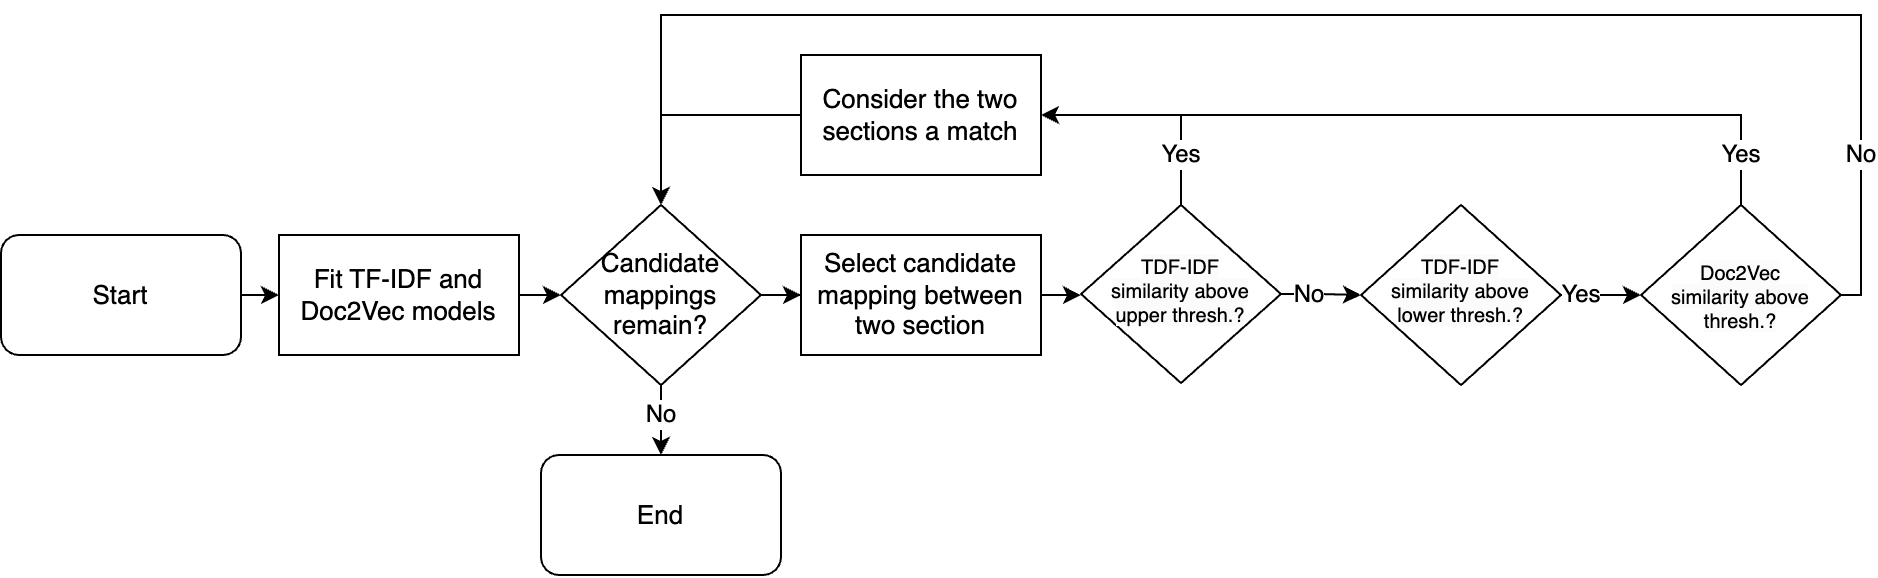
\includegraphics[width=1\textwidth]{hybrid-model-horizontal.png}}
\label{fig:hybrid-model}
\end{figure*}

\method{Clustering}
Another approach to measure the similarity of sections was to cluster sections based on their `tags'. A tag could be a concept's name or subject, as defined in Section~\ref{sec:modelling-of-textbooks}. A similar approach, whereby the content of textbooks is represented at the level of domain concepts rather than using the literal content is explored in \textcite{thaker2018}. In this research, K-means clustering is used.

Each section is represented as a binary vector, where each element indicates the presence or absence of a particular tag. Sections are clustered based on these vectors. The similarity score between two sections is binary and determined by whether two sections are in the same cluster. In the case that multiple attributes are used, the weighted average of these binary outcomes is taken, to achieve a continuous similarity score that is tested against a minimum threshold to ensure that sections can be considered similar.

\begin{itemize}
    \bolditem{Section Attributes} The attribute(s) that the sections are clustered on. \quad$\mathcal{P}\left(\{\text{concept name}, \text{concept category}\}\right)$.
    \bolditem{Number of Clusters} A hyperparameter of the K-means clustering algorithm. When clustering is performed multiple times (i.e. multiple section attributes are used), the number of clusters parameter must be set as many times as a clustering algorithm is run (e.g. for two section attributes, use two values of the number of clusters parameter). \quad$\{40, 60, 80, 100, 120\}$
    \bolditem{Threshold} A minimum similarity score to consider two sections a match. Only used for multiple section attributes, as described above. \quad$\{0.2, 0.4, 0.6\}$
    \bolditem{Weights} How much weight to give each attribute when taking the weighted average of similarity scores (for multiple attributes only). \quad$\left\{X \in \mathcal{P}\left(\{0.2,0.4,0.6,0.8\}\right) \mid \left|X\right| = 2 \right\}$
\end{itemize}


\method{TF-IDF \& Clustering Ensemble Averaging}
It is known that ensemble algorithms perform better than their singular counterparts \cite{opitz1999}. This is based on the common societal practice of `seeking a second opinion' \cite{polikar2006}. Thus, Methods A \& C were combined to form an ensemble model. The parameters of each of these methods are used in the same way in this ensemble approach.


\method{TF-IDF \& Doc2Vec Iterative Hybrid}
Similarly, it was observed that the Doc2Vec and TF-IDF models have different strengths and weaknesses. For example, TF-IDF had better precision while Doc2Vec had better recall. TF-IDF can observe exact matches in attributes of the section that are less likely to have synonyms (e.g. the header or concepts), while Doc2Vec can observe similarities in the textual content, which might be worded in any number of ways. Thus, a hybrid approach was implemented whereby the models are combined iteratively. Based on cosine similarity thresholds, the TF-IDF model first classifies some matches between sections as `definitive', while maintaining a record of some `uncertain' matches. Simultaneously a Doc2Vec model is fit. Matches that are within the uncertain thresholds for the first model are then checked against the Doc2Vec model to see if they have a score above the Doc2Vec threshold. These matches are added to the resulting integration of sections.

This approach uses the same parameters that are used in Methods A \& B. Additionally, there is a new parameter, ``Uncertain Threshold'', that provides a minimum TF-IDF similarity score value for a match to be included. If a match scores above this value, but below the TF-IDF standard threshold, the match's similarity score in the Doc2Vec model will be checked to see whether it would be considered a match within the Doc2Vec framework, essentially given the potential match a `second chance'. This process is described by the flowchart in Figure~\ref{fig:hybrid-model}.


\subsubsection{Converting Integrated Textbook to Labelled Dataset} \label{sec:converting-to-labelled-dataset}
Once the textbooks are integrated using the optimal method, it is necessary to convert the newly created hierarchy of textbook sections into a normalised, labelled dataset that can be used for supervised machine learning. We perform this conversion by taking each section (and all their attributes) to be a single instance in our dataset. Then, the class label is set to be the section's largest ancestor.

\begin{figure*}[h!]
\caption{Example conversion from integrated textbook's hierarchy of sections to normalised labelled dataset}
\centerimg{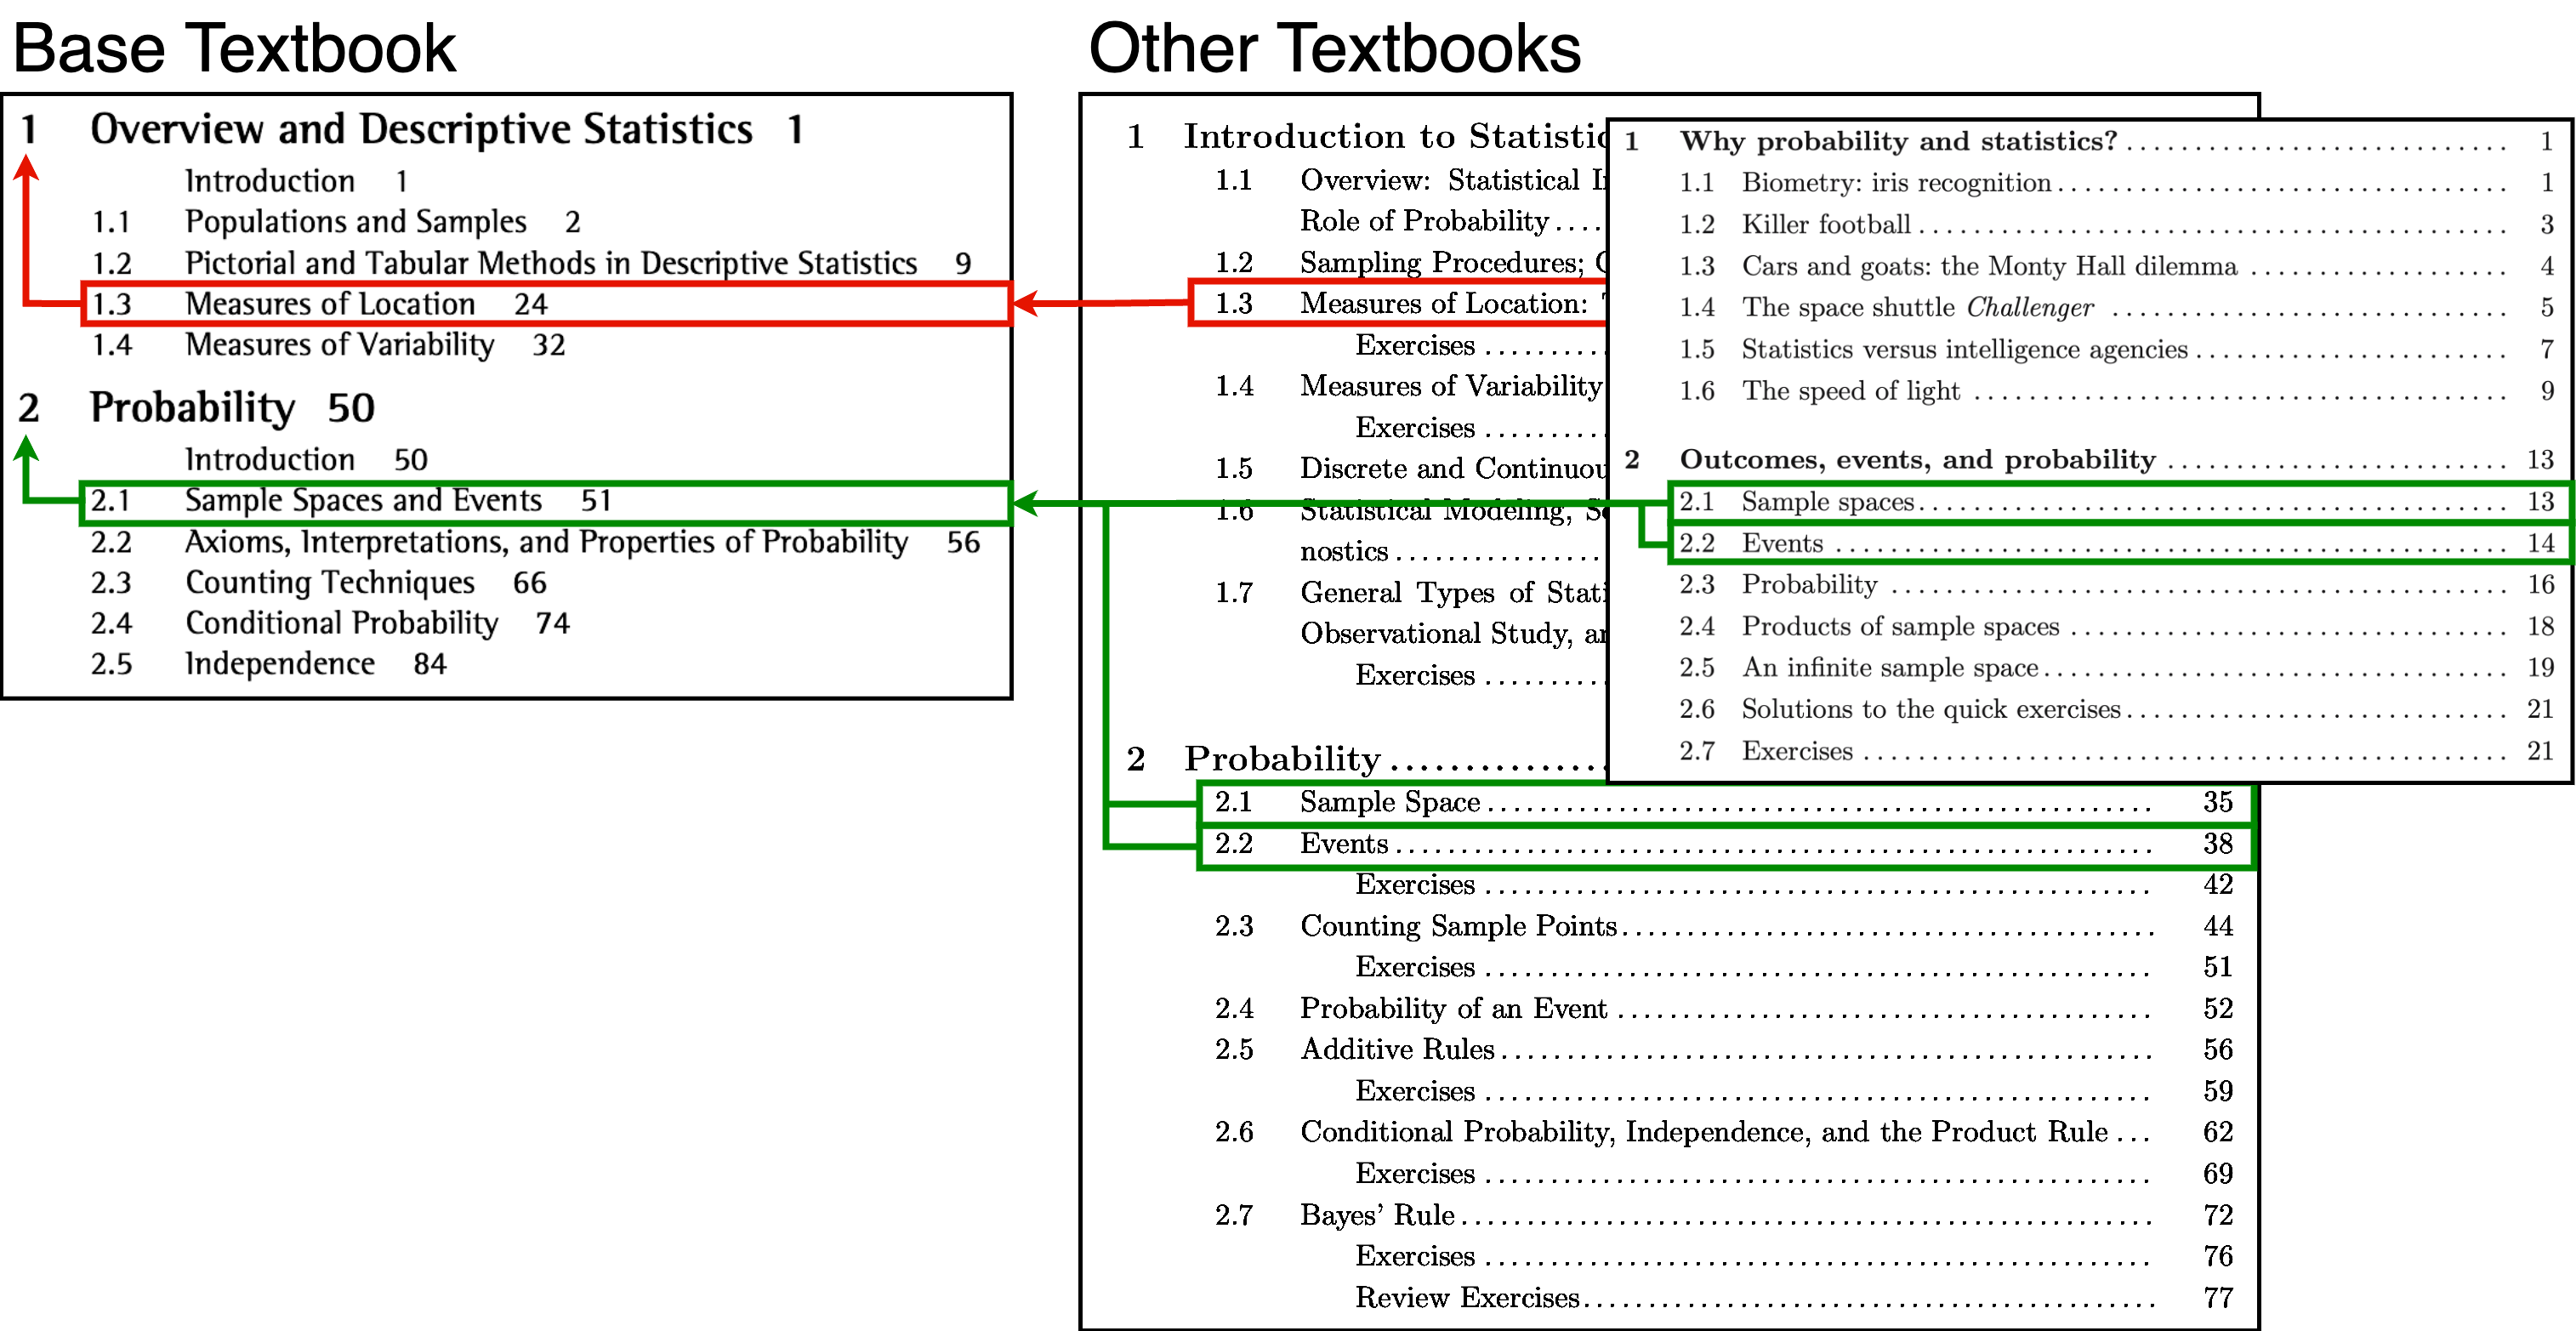
\includegraphics[width=0.9\textwidth]{integration.png}}
\label{fig:integration}
\end{figure*}

Consider Figure~\ref{fig:integration} as an example of this approach. In the diagram, there are seven highlighted sections across three textbooks. However, these fit into only two class labels (“Overview and Descriptive Statistics” and “Probability”) since these are the top-level sections from the base textbook. This approach is taken to ensure that each class has sufficient membership.

From the previous methods, the optimal method is used to generate two hierarchical topic models to convert to labelled datasets. The first, known hereafter as ``small'', is generated by using the optimal method to integrate the same two textbooks that were used to evaluate the textbook integration methods (\code{BookA} and \code{BookB}). The second dataset (``large'') is generated by using the optimal method to integrate all twelve textbooks. Additionally, the expert's manual hierarchy of topics, described in Section~\ref{sec:results-stage-1}, is used to generate a third ``expert'' dataset.

\subsection{Phase 2: Topic Classification} \label{sec:topic-classification}
Once the three new datasets have been generated, they are used to train an advanced language model for the classification task. 

First, vector embeddings for each textbook section are obtained using BERT. BERT accepts special tokens (\code{[CLS]} and \code{[SEP]}) which can be used to provide the model with two different features of the input sequence, so we test two approaches. In the first approach, concept names are prepended to the section’s content, while the second approach simply uses the section’s content. Consider the following example BERT tokenisation input where concepts are prepended to the input sequence for a section titled ``Measures of Variability'' :

\begin{quotation}\noindent\small
\code{[CLS]}
Degrees of freedom \enspace
Population \enspace
Parameter \enspace
Range \enspace
Standard deviation \enspace
Variance \enspace
Population
\code{[SEP]}
Sample variability plays an important role in data analysis. Process and product variability is a fact of life in engineering and scientific systems: The control or reduction of process variability is often a source ...
\code{[SEP]}
\end{quotation}

This approach is similar to the approach to BERT input encoding taken in \textcite{alpizarchacon2023a}: concept names are used to summarise the section's textual content.

We propose that this addition allows the model to differentiate between the two different kinds of information and learn how concepts are described by the content, enhancing its ability to understand and represent the relationship between these two elements in the text. This proposal is explored as a part of \textbf{RQ2}.

The input text is then tokenized and truncated or padded to ensure that the length of each input is exactly 512 tokens. To convert input tokens to fixed-size tensors, the inputs must be the same length. One approach is to pad all sequences with a special token (usually $0$) so that each sequence is the same length as the longest sequence in the batch. However, due to the Transformer network architecture of BERT, its time complexity involves a quadratic dependency of the sequence length \cite{vaswani2017}. Therefore, to avoid degraded performance, a token limit of 512 is set and all sequences with more tokens are truncated. It is proposed that the content of a textbook section might be effectively summarised by the first 512 tokens since textbooks typically include an all-encompassing introduction at the beginning of sections and subsections. Thus, it is assumed that minimal information will be lost through the truncation process.

Once the input is tokenised, it is passed to the pre-trained DistilBERT model\footnote{from the Hugging Face transformers library \cite{huggingface}}, which converts the text into a high-dimensional vector representing various linguistic features. In this research, no fine-tuning is performed on top of the pre-trained BERT model, since this would require a labelled dataset. While our dataset does have labels, these labels will be used later to train RNNs for classification. Fine-tuning the BERT model using these labels will result in data leakage, i.e. the training data for our RNNs will contain information about the targets.

These vectors are then used to train RNNs to classify new sections according to their topic. It’s important to note that the class label originates from the largest ancestor of the section in the integrated textbook. In other words, if the section comes from the base textbook, the class label is the top-level section that it belongs to. If the section comes from the other textbooks, its class label is the top-level section that its base textbook match belongs to. This approach is taken to ensure that each class has enough members.

Additionally, there are parameters available to be chosen for RNNs:

\begin{itemize}
    \bolditem{Batch Size $(N)$} the number of training examples used in one iteration of model training (i.e. used to compute the gradient and update the model parameters).
    \bolditem{Dropout Rate $(p)$} the probability of an input unit being dropped or set to zero during training. This helps prevent overfitting by forcing the network to learn redundant representations.
    \bolditem{Units $(u)$} the number of units or neurons in a layer.
\end{itemize}

To select the optimal parameters for the neural network, a grid search with 5-fold cross-validation was performed. As part of the grid search, we also varied the model type between RNN and LSTM.

Accuracy is chosen as the key metric to optimise and evaluate models. This is because it is a direct reflection of the number of correct predictions and, particularly in the case of multi-class classification, it is simple and easy to interpret.

For each dataset, we performed the grid search twice. This was to test the model’s performance when concepts were both included and omitted from the input text, allowing us to explore \textbf{RQ2}.

\begin{table*}
\centering
\caption{Results of optimal model for each textbook integration method}
\label{table:phase1-results}
\begin{tabular}{lccccccc}
\toprule
method & TP & FP & FN & precision & recall & $F_1$ & $F_\beta$ \\
\midrule
A & 48 & 33 & 94 & 0.593 & 0.338 & 0.430 & 0.515 \\
B & 56 & 42 & 86 & 0.571 & \textbf{0.394} & \textbf{0.467} & 0.524 \\
C & 4 & 150 & 138 & 0.026 & 0.028 & 0.027 & 0.026 \\
D & 44 & 51 & 98 & 0.463 & 0.310 & 0.371 & 0.421 \\
E & 45 & 9 & 97 & \textbf{0.833} & 0.317 & 0.459 & \textbf{0.628} \\
\bottomrule
\end{tabular}
\end{table*}


\section{Results \& Evaluation} \label{sec:results}

This section presents the results that were seen when testing our proposed methodology. Additionally, we attempt to answer our research questions with a greater level of certainty by using statistical hypothesis testing. For all statistical tests, the level of significance is $\alpha=0.05$. Furthermore, the p-values are adjusted using the Bonferroni correction to avoid the multiple comparisons problem.

\subsection{Phase 1: Dataset Generation}\label{sec:results-stage-1}

To evaluate the performance of the textbook integration task, we used a ``ground truth'' produced by three experts from Utrecht University for previous research \cite{alpizarchacon2020}. This data consists of a manual mapping between the chapters, sections, and subsections of \code{BookA} to those of \code{BookB}. Experts had the flexibility to link textbook sections at various levels within the table of contents, allowing for many-to-many mappings. They were also asked to specify the strength of the mappings on a scale from one to three, however, this additional information was not used in this research. 

It is important to note that, given the expert ground truth only exists for mappings between two of the textbooks, it is impossible to evaluate the textbook linkage performance on the entire dataset. One possible implication is that the best textbook integration method is selected based on the integration of two textbooks, and such a method might not be able to be effectively extended to the integration of twelve textbooks.

The standard precision and recall metrics were used to compare the performance of the different textbook linking algorithms. In this context, precision is the proportion of the mappings identified by the algorithm that the experts also identify. Recall is the proportion of the mappings identified by the experts that the algorithm also identifies.

While both metrics are important, it can be argued that precision is the more important metric of the pair in the domain of online education. While both false positives and false negatives are undesirable, in many educational contexts, the cost of a false positive (e.g. wrongly associating two topics) can have greater cost than a false negative (e.g. failing to identify a similarity between two topics). Precision focuses on minimising false positives.

However, it is important to note that this does not mean recall is unimportant, especially since the downstream uses of this research are not yet specified in detail. A balanced approach that considers both precision and recall is often the best strategy, especially in scenarios where missing out on key information (low recall) could be as detrimental as providing incorrect information (low precision). 

Thus, it was decided to use the $F_\beta$ score for evaluation, which is the weighted harmonic mean of precision and recall. The $\beta$ parameter represents the importance of recall over precision, such that $\beta=0.5$ means that we consider recall to be half as important as precision \cite{rijsbergen1979}. The formula for the $F_\beta$ score is shown in Equation~\ref{eq:fbeta}.

\begin{equation}\label{eq:fbeta}
% F_\beta = \frac{ (1 + \beta^2) \times \text{true positives} }{ (1 + \beta^2) \times \text{true positives} + \beta^2 \times \text{false negatives} + \text{false positives} }
F_\beta = (1 + \beta^2)\cdot\frac{\text{precision}\cdot\text{recall}}{\beta^2\cdot\text{precision}+\text{recall}}
\end{equation}

For each integration strategy, we performed a grid search to find the optimal parameter choices. This led to 984 different combinations of parameters and algorithms. Table~\ref{table:phase1-results} shows the results of the best-performing parameter combinations for each textbook integration method.

Out of the individual models, Method A and Method B seem to be the best performing. Given that Method E improves on the results of these models, with particularly good precision, the approach of combining Methods A \& B seems to be successful.

It should be noted that the iterative approach described previously did not yield the best results for any of the strategies, but it did result in a significant increase in computation time.

To determine whether Method E has a statistically significant advantage over the other methods according to the $F_\beta$ score (and thus answer \textbf{RQ1}), a Mann–Whitney $U$ test was performed with the following null hypothesis:
\nullhypothesis{
    The distribution underlying the $F_\beta$ scores for Method E is not stochastically greater than the distributions underlying the $F_\beta$ scores for the other methods.
}
\begin{table}[h!]
\centering
\caption{Results of Mann–Whitney $U$ test for \textbf{RQ1}}
\label{table:rq1-statistical-tests}
\begin{threeparttable}
\begin{tabular}{cccccc}
\toprule
method & $\mu$ & $\sigma$ & $U$ & adj.\,$p$ \\
\midrule
A & 0.363 & 0.120 & 9981.0 & \sig \\
B & 0.276 & 0.124 & 25491.5 & \sig \\
C & 0.008 & 0.008 & 33120.0 & \sig \\
D & 0.136 & 0.083 & 48335.0 & \sig \\
\midrule
E & 0.484 & 0.054 & – & – \\
\bottomrule
\end{tabular}
\begin{tablenotes} \footnotesize\centering
\nonumitem \sig\ indicates $p \leq 0.001$
\end{tablenotes}
\end{threeparttable}
\end{table}



The Mann–Whitney $U$ test is the optimal statistical test in this scenario since the samples are not paired and the Shapiro–Wilk test shows that the data is not normally distributed. The results of this test are shown in Table~\ref{table:rq1-statistical-tests}. The results are statistically significant, allowing us to reject the null hypothesis. Thus, Method E is statistically more performant than the other methods, answering \textbf{RQ1}.

Thus, Method E (TF-IDF \& Doc2Vec Iterative Hybrid model) is used in the next phase. The optimal parameters and attributes to be used with this method are as follows:

\begin{itemize} \itemsep-0.2em
    \bolditem{TF-IDF Section Attributes} $\{\text{content}, \text{concept names}\}$
    \bolditem{TF-IDF Upper Threshold} $0.6$
    \bolditem{TF-IDF Lower Threshold} $0.3$
    \bolditem{Doc2Vec Section Attribute} content
    \bolditem{Doc2Vec Threshold} $0.6$
    \bolditem{Doc2Vec Vector Size} $100$
    \bolditem{Doc2Vec Minimum Count} $1$
\end{itemize}

This Method E was then used to generate two hierarchical topic models (``small'' and ``large'', as described in Section~\ref{sec:converting-to-labelled-dataset}), which are then converted to labelled datasets. Additionally, the expert's manual hierarchy of topics is also converted to a labelled dataset. Table~\ref{table:generated-dataset-features} displays some features of these datasets.

\begin{table}[h!]
\centering
\caption{Features of generated datasets}
\label{table:generated-dataset-features}
\begin{tabular}{cccccc}
\toprule
dataset & instances & topic labels \\
\midrule
small & 354 & 32  \\
large & 2368 & 329  \\
expert & 216 & 14  \\
\bottomrule
\end{tabular}
\end{table}

\subsection{Phase 2: Topic Classification}

As outlined in Section~\ref{sec:converting-to-labelled-dataset}, three different datasets (generated using the process described in Phase 1) were used to train and evaluate the neural networks in this stage. Additionally, the classification models were tested both with and without concepts prepended to the sequence. The optimal models that were found in each grid search are displayed in Table~\ref{table:phase-2-results-a}.

\begin{table}[h]
\centering
\caption{Selected parameters for each dataset}
\label{table:phase-2-results-a}
\begin{tabular}{lllrrr}
\toprule
dataset & concepts & model & $N$ & $p$ & $u$ \\
\midrule
expert & true & SimpleRNN & 128 & 0.4 & 125 \\
expert & false & LSTM & 128 & 0.4 & 200 \\
small & true & SimpleRNN & 32 & 0.9 & 100 \\
small & false & SimpleRNN & 64 & 0.9 & 100 \\
large & true & SimpleRNN & 64 & 0.9 & 125 \\
large & false & SimpleRNN & 64 & 0.9 & 100 \\
\bottomrule
\end{tabular}
\end{table}


\begin{table*}[h]
\centering
\begin{threeparttable}
\caption{Test performance of the optimal model for each dataset}
\label{table:phase2-results-b}
\begin{tabular}{lccccccccc}
\toprule
\multirow{2}{*}{dataset} & \multirow{2}{*}{concepts} & \multicolumn{2}{c}{accuracy} & \multicolumn{2}{c}{precision} & \multicolumn{2}{c}{$F_1$} \\
 &  & model & baseline & model & baseline & model & baseline \\
\midrule
expert & true & \textbf{0.59} & 0.13 & \textbf{0.67} & 0.07 & 0.61 & 0.08 \\
expert & false & 0.41 & 0.13 & 0.50 & 0.09 & 0.44 & 0.09 \\
small & true & 0.35 & 0.03 & 0.48 & 0.01 & 0.53 & 0.02 \\
small & false & 0.45 & 0.03 & 0.64 & 0.01 & \textbf{0.62} & 0.02 \\
large & true & 0.26 & 0.00 & 0.56 & 0.00 & 0.40 & 0.00 \\
large & false & 0.24 & 0.00 & 0.57 & 0.00 & 0.37 & 0.00 \\
\bottomrule
\end{tabular}
\begin{tablenotes} \footnotesize\centering
\nonumitem Recall is excluded because weighted-average recall is equivalent to accuracy for multiclass classification. Weighted-average precision is used.
\end{tablenotes}
\end{threeparttable}
\end{table*}





For each of these optimal models, we compared the performance of the model to that of a baseline, chosen to be BERTopic\footnote{\url{https://github.com/MaartenGr/BERTopic}}\cite{grootendorst2022}. BERTopic is a topic modelling framework based on BERT that has several capabilities, including out-of-the-box topic classification. It was chosen as a baseline due to its ease of use as well as its robust performance across a variety of tasks.

The performance of the optimal models for each dataset, as well as the baseline performance, are displayed in Table~\ref{table:phase2-results-b}. The results presented are the average of 5-fold cross-validation. In every metric, our models perform better than the BERTopic baseline.

Additionally, across the expert and large datasets, our model performs better when concepts are prepended to the input text. Statistical tests, using the following null hypothesis, were performed to confirm this and thus answer \textbf{RQ2}.

\nullhypothesis{
    The distribution of accuracy scores is not stochastically greater when including concepts in the input embeddings.
}

The Shapiro–Wilk test confirmed that the data was normally distributed, allowing the use of the paired samples $t$-test. In this test, the paired samples are the accuracy scores achieved under the same conditions both with and without the inclusion of concepts. The results, displayed in Table~\ref{table:rq2-statistical-tests}, are statistically significant for the expert and large datasets. Therefore, for these datasets, we can reject the null hypothesis that there is no improvement in accuracy when concepts are included in the input embeddings.

\begin{table}[h!]
\centering
\begin{threeparttable}
\caption{Results of paired samples $t$-test for \textbf{RQ2}}
\label{table:rq2-statistical-tests}
\begin{tabular}{lcccc}
\toprule
dataset & $\mu$ & $\sigma$ & $t$ & adj.\,$p$ \\
\midrule
expert & 0.015 & 0.026 & 5.801 & \sig \\
small & 0.003 & 0.017 & 1.599 & 0.170 \\
large & 0.006 & 0.008 & 4.117 & \sig \\
\bottomrule
\end{tabular}
\begin{tablenotes} \footnotesize\centering
\nonumitem \sig\ indicates $p \leq 0.001$
\end{tablenotes}
\end{threeparttable}
\end{table}



Additionally, the expert dataset performs better than the generated datasets and the large, generated dataset performs particularly badly. This might be due to the large number of classes introduced by integrating all twelve textbooks simultaneously.

Statistical tests were performed to confirm whether the expert dataset results in the best performance across all metrics. The data is not normally distributed (as confirmed by the Shapiro–Wilk test), therefore, the Mann–Whitney $U$ test was used with the following null hypothesis:

\nullhypothesis{
    The distribution of accuracy scores for classification using the expert dataset is not stochastically greater than the metrics achieved on the large and small datasets.
}

\begin{table*}[h!]
\centering
\caption{Results of Mann–Whitney $U$ test for \textbf{RQ3}}
\label{table:rq3-statistical-tests}
\begin{threeparttable}
\begin{tabular}{cccccccccccccccccccc}
\toprule
\multirow{2}{*}{dataset} & \multicolumn{4}{c}{with concepts} &  & \multicolumn{4}{c}{without concepts} \\
\hhline{~----~----}
  & $\mu$ & $\sigma$ & $U$ & adj.\,$p$ &  & $\mu$ & $\sigma$ & $U$ & adj.\,$p$ \\
\midrule
large & 0.25 & 0.03 & 2304.0 & \sig &  & 0.24 & 0.03 & 2304.0 & \sig \\
small & 0.30 & 0.01 & 9216.0 & \sig &  & 0.30 & 0.02 & 9216.0 & \sig \\
\midrule
expert & 0.52 & 0.03 & – & – &  & 0.51 & 0.03 & – & – \\
\bottomrule
\end{tabular}
\begin{tablenotes} \footnotesize\centering
\nonumitem \sig\ indicates $p \leq 0.001$
\end{tablenotes}
\end{threeparttable}
\end{table*}



The results are displayed in Table~\ref{table:rq3-statistical-tests}. All of the adjusted p-values are significant, allowing us to reject the null hypothesis. Therefore, answering \textbf{RQ3}, we can say with some certainty that the manually-generated expert dataset performs better at the topic classification task than the datasets that were automatically generated using our optimal content linkage method.

\section{Discussion \& Limitations} \label{sec:discussion}
% Discuss results, implications, limitations, and review research questions

Overall, this research has shown that extracting fine-grained, domain-specific topic models from textbooks is effective. While there are obvious limitations in many parts of our proposed architecture, these could be resolved in future research, with tremendous implications for the facilitation of tasks such as learning object classification, automatic index creation, and content personalisation.

When comparing the textbook integration techniques used in Phase 1 for \textbf{RQ1}, it is interesting to note that a combination of two individual approaches is the best performing (i.e. the combination of Methods A \& B resulting in Method E). This is in line with expectations that ensemble learning results in performance improvements. However, it is important to note that combining two models to form an ensemble model results in significant increases in computation time. Further research might explore how these methods might be optimised or combined more efficiently.

Furthermore, when converting the generated hierarchy of topics into a labelled dataset (described in  Section~\ref{sec:converting-to-labelled-dataset}), it was decided to take a section's topic label as its largest ancestor in the hierarchy. This likely results in a less fine-grained model than if a more precise topic label were taken (e.g. from the second or third largest ancestor). While this results in additional complexities, such as low class membership counts, further research might explore how these can be mitigated to create topic models that possess even finer granularity.

For \textbf{RQ2}, the inclusion of concept annotations significantly improved model performance for the large and expert datasets. It should also be noted that this performance is using a pre-trained DistilBERT implementation without fine-tuning. Perhaps with more time or resources, a model that is more customised to our use case could be fine-tuned. An alternative approach that might also be explored in future research is the use of a fine-tuned BERT model for classification instead of using RNNs trained on BERT embeddings.

Additionally, the way that we have used the BERT special tokens is not entirely consistent with the intended usage for the pre-trained BERT and DistilBERT models. Specifically, the \code{[SEP]} token is intended to separate the tokens into two sentences for the NSP task. However, when we prepend concepts to the input, the first `sentence' in our input is not a true sentence but rather a list of words that do not make sense when strung together as a sentence (e.g. ``Degrees of freedom Population Parameter Range Standard deviation Variance Population''). With more time and resources, a custom implementation of BERT might be pre-trained so that the first sentence of the input is more syntactically alike to our first sentences.

Furthermore, due to constraints in computing time and resources, only the first 512 tokens of each input sequence were passed to the BERT. It might be the case that this small part of the text is inadequate at capturing the full meaning of each textbook section. Therefore, performance benefits might be seen if the maximum number of tokens for the input sequence is increased, or if longer sequences are split to form a larger dataset.

Also, the investigation into \textbf{RQ3} revealed that the quality of datasets plays a crucial role, with higher quality datasets leading to improved performance of machine learning models. The strong performance of the expert dataset in the topic classification tasks allows us to assume that if we improve the textbook integration in Phase 1, we might be able to improve the performance of topic classification on the generated dataset in Phase 2.

Additionally, in this research, the Python programming language has been used to allow for the fast development of a proof of concept. Python was an effective choice in achieving this goal, due to its simplicity, readability, and the vast availability of libraries and frameworks to streamline the development process. 
However, Python's interpreted nature can make it less efficient for fast or high-performance machine learning tasks compared to languages that are compiled and optimised for speed. Additionally, Python is limited in its multi-threaded execution capabilities, meaning there are limited gains to be achieved by executing independent code in parallel. Future research might focus more on increasing the speed and efficiency of the code so that more powerful models can be used, or the models can be applied to a larger dataset.

There were minimal ethical impacts concerning this research since the research does not involve humans and there are no immediately obvious negative uses or consequences of this research. The data being used does not contain any Personal Identifiable Information. While a general ethical consideration for AI models is that they may inadvertently learn and perpetuate biases in their training data, this concern is mitigated by the fact that the data consists of scientific textbooks, which are generally considered to be very unbiased sources of information.

Our research marks a significant development towards personalised learning, where educational applications can be customised to meet the unique needs and learning paths of individuals. Accurately constructing domain models from textbooks provides a robust framework for various tasks that can improve the overall educational experience. Therefore, this research not only contributes to the academic discourse on AI's role in education but also paves the way for practical applications in personalised learning environments.

\section{Conclusion} \label{sec:conclusion}
In this research, we have presented a novel architecture for the classification of topics in educational content, focusing on the extraction of domain-specific and fine-grained topic models from textbooks. Our work takes a significant step forward in applying artificial intelligence to enhance the digital learning experience, addressing the challenge of accurately classifying and linking educational content across various domains. The performance of this architecture is not strong enough for use in production applications; however, the initial results give promise that further research and investments in computing power might yield a pipeline that can generate more correct data and classify new data more accurately.

The implementation of the first phase of our architecture revealed the significant complexity inherent in developing an efficient and performant content linkage tool. Despite limitations due to the availability of expert mappings for only a subset of textbooks, our comparison of textbook linking algorithms provided insightful data on the effectiveness of these methods. Our results indicate that a TF-IDF \& Doc2Vec Iterative Hybrid model, showed reasonably high levels of precision, suggesting a promising approach for integrating textbook content.

In Phase 2, our RNN models trained on BERT embeddings demonstrated improved performance across all metrics compared to the BERTopic baseline, particularly when concept annotations were prepended to the input text. This suggests that the inclusion of domain-specific concepts significantly enhances model accuracy, especially for the expert and large datasets, validating our approach to model training.

Although challenges remain, such as the moderate performance of our automatic content linkage method compared to expert manual efforts, our approach to topic classification shows promise. Our findings underscore the importance of using high data quality to optimise the performance of advanced machine learning models in classifying textbook content. The reasonably strong performance of topic classification on the expert dataset illustrates that, if accurately generated, topic models constructed from textbooks can accurately reflect the depth and breadth of subjects and thus result in a strong performance when used as inputs into domain-specific and fine-grained topic classification.

Our research has demonstrated the potential of leveraging the intricate knowledge embedded in textbooks in conjunction with advanced AI and NLP techniques in revolutionising the online learning experience. By adopting a methodical approach to extract and utilise fine-grained, domain-specific topic models, we have uncovered insights that not only answer our primary research question regarding the efficacy of machine learning methods in this context but also pave the way for future innovations in educational technology, such as improved searchability, personalization, and recommendation systems in online learning systems.

Future research must continue to explore and refine AI-based educational tools, focusing on overcoming current limitations and enhancing the efficacy of topic models. Constraints relating to computing time and resources are the key limitations that should be explored in future research. By harnessing the power of domain-specific, fine-grained topic modelling, we move closer to realising the vision of a more efficient, effective, and accessible educational system for learners.

The code for this research is available in a public \href{https://github.com/CobySim01/textbook-topic-analysis}{GitHub repository}\footnote{\url{https://github.com/CobySim01/textbook-topic-analysis}}.


\small\printbibliography

\end{document}
